%*******************************************************************************
%*********************************** First Chapter *****************************
%*******************************************************************************

\chapter{GIỚI THIỆU}  %Title of the First Chapter

\ifpdf
    \graphicspath{{Chapter1/Figs/Raster/}{Chapter1/Figs/PDF/}{Chapter1/Figs/}}
\else
    \graphicspath{{Chapter1/Figs/Vector/}{Chapter1/Figs/}}
\fi


%********************************** %First Section  **************************************
\section{Ý tưởng và tính cấp thiết của đề tài}\label{section1.1}

Ngày nay, bài toán giao thông vẫn đang là bài toán hóc búa vẫn chưa được giải quyết được ở Việt Nam và nhiều nước đang phát triển. Tình trạng kẹt xe, ùn tắc kéo dài gây ra sự chậm trễ trong công việc, hơn nữa còn  gây gia tăng ô nhiễm môi trường, giảm chất lượng môi trường sống. Một trong những khó khăn làm bài toán giao thông khó giải quyết đó chính là không có đầy đủ dữ liệu cần thiết. Chúng ta không thể giải bài toán nếu không có đủ dữ kiện, cũng như giải quyết kẹt xe ta cần phải có dữ liệu về lưu lượng giao thông.

Vì yếu tố trên, dự án Smart Traffic được hình thành và phát triển theo hướng IoT với mục đích thu thập dữ liệu về các yếu tố môi trường (nồng độ CO, nhiệt độ, độ ẩm, nồng độ bụi, độ ồn…) và xác định mối tương quan giữa lưu lượng giao thông với môi trường xung quanh khu vực đó. Từ đó ta có thể có được 1 phần dữ liệu cần thiết về tình trạng các con đường theo thời gian thực, cũng như có được lịch sử và dùng dữ liệu ấy để phát triển dự đoán tình trạng giao thông tiếp theo.

\begin{figure}[H] 
\centering    
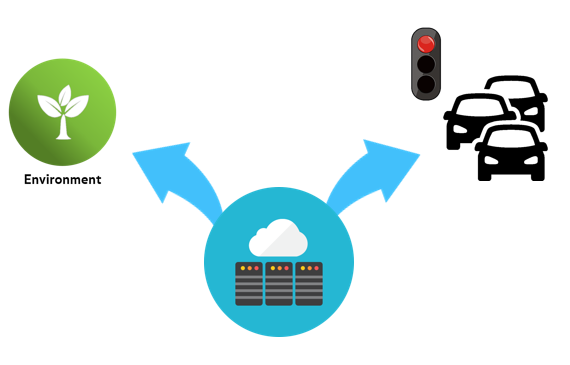
\includegraphics[width=1.0\textwidth]{pic1}
\caption[Mô hình ứng dụng dữ liệu của đề tài]{Mô hình ứng dụng dữ liệu của đề tài}
\label{fig:pic1}
\end{figure}

Những dữ liệu đó có thể được phân tích và xử lý, đưa ra những kết luận về tình trạng lưu thông trên đoạn đường đó, về sự thay đổi môi trường tại 1 khu vực ở những khoảng thời gian khác nhau. Và những dữ liệu này có thể ứng dụng cho bất động sản, môi trường và nghiên cứu. Do đó đề tài mang tính thiết thực và ứng dụng cao và được lựa chọn để làm Thực tập tốt nghiệp và có thể lên Luận văn tốt nghiệp.




\section{Mục tiêu và nhiệm vụ của đề tài} %Section - 1.1 
\label{section1.2}
\subsection{Mục tiêu đề tài}
\begin{itemize}
\item[-]Tìm hiểu về khí thải xe máy và ô tô.

\item[-]Hiện thực mạch cảm biến để thu thập khí thải.

\item[-]Khảo sát và đo khí thải thực tế tại một số điểm thường xuyên xảy ra kẹt xe trên địa bàn thành phố.

\item[-]Tổng hợp các số liệu thu thập và các yếu tố môi trường khác (nhiệt độ, độ ẩm, …) để đề xuất mô hình để hướng đến phát triển hệ thống cảnh báo kẹt xe dựa vào tình trạng ô nhiễm không khí.

\item[-]Hiện thực hoàn module thu thập cảm biến tích hợp thêm module sử dụng năng lượng mặt trời để nạp pin cho mạch hoạt động độc lập với điện lưới.
\item[-]Hoàn chỉnh website cho phép người dùng theo dõi thông tin.
\item[-]Đề xuất các tính năng thừa hưởng từ kết quả hệ thống và khả năng tích hợp với các hệ thống khác.


\end{itemize}

\subsection{Nhiệm vụ đề tài}

\begin{landscape}
\begin{table}[]
\centering
\caption{Giản đồ gantt của Huỳnh Phạm So Ny}
\label{my-label}
\begin{tabular}{|l|l|l|l|l|l|l|l|l|l|l|l|l|l|l|l|l|}
\hline
\multicolumn{1}{|c|}{}                      & \multicolumn{1}{c|}{}                                                                             & \multicolumn{15}{c|}{Tuần}                                                                                                                                                                                                                                                                                                                                                                                                                \\ \cline{3-17} 
\multicolumn{1}{|c|}{\multirow{-2}{*}{STT}} & \multicolumn{1}{c|}{\multirow{-2}{*}{Công việc}}                                                  & 1                        & 2                                               & 3                        & 4                        & 5                        & 6                        & 7                        & 8                        & 9                        & 10                       & 11                       & 12                       & 13                       & 14                       & 15                       \\ \hline
1                                           & \begin{tabular}[c]{@{}l@{}}Tìm hiểu các thiết,bị sensor, MCU, \\ Module SIM\end{tabular}          & \cellcolor[HTML]{000000} & \cellcolor[HTML]{000000}                        & \cellcolor[HTML]{000000} &                          &                          &                          &                          &                          &                          &                          &                          &                          &                          &                          &                          \\ \hline
2                                           & Tìm hiểu về pin,năng lượng mặt trời                                                               &                          & \cellcolor[HTML]{000000}{\color[HTML]{000000} } &                          &                          &                          &                          &                          &                          &                          &                          &                          &                          &                          &                          &                          \\ \hline
3                                           & Làm prototype đầu tiên                                                                            &                          &                                                 &                          & \cellcolor[HTML]{000000} &                          &                          &                          &                          &                          &                          &                          &                          &                          &                          &                          \\ \hline
4                                           & Suy nghĩ design,tổng thể cho cái hộp                                                              &                          &                                                 & \cellcolor[HTML]{000000} & \cellcolor[HTML]{000000} & \cellcolor[HTML]{000000} &                          &                          &                          &                          &                          &                          &                          &                          &                          &                          \\ \hline
5                                           & Thiết kế bản vẽ cho,hộp                                                                           &                          &                                                 &                          &                          &                          & \cellcolor[HTML]{000000} &                          &                          &                          &                          &                          &                          &                          &                          &                          \\ \hline
6                                           & Coding                                                                                            &                          &                                                 &                          &                          &                          & \cellcolor[HTML]{000000} &                          &                          &                          &                          &                          &                          &                          &                          &                          \\ \hline
7                                           & Thiết kế PCB cho,mạch                                                                             &                          &                                                 &                          &                          &                          & \cellcolor[HTML]{000000} & \cellcolor[HTML]{000000} &                          &                          &                          &                          &                          &                          &                          &                          \\ \hline
8                                           & \begin{tabular}[c]{@{}l@{}}Hoàn thiện node cảm biến chạy bằng \\ năng lượng mặt trời\end{tabular} &                          &                                                 &                          &                          &                          &                          & \cellcolor[HTML]{000000} & \cellcolor[HTML]{000000} &                          &                          &                          &                          &                          &                          &                          \\ \hline
9                                           & Testing                                                                                           &                          &                                                 &                          &                          &                          &                          &                          &                          & \cellcolor[HTML]{000000} & \cellcolor[HTML]{000000} & \cellcolor[HTML]{000000} &                          &                          &                          &                          \\ \hline
10                                          & Chọn lại Module SIM và redesign lại PCB                                                           &                          &                                                 &                          &                          &                          &                          &                          &                          &                          &                          & \cellcolor[HTML]{000000} &                          &                          &                          &                          \\ \hline
11                                          & Nhân bản ra 2 node,cảm biến                                                                       &                          &                                                 &                          &                          &                          &                          &                          &                          &                          &                          & \cellcolor[HTML]{000000} & \cellcolor[HTML]{000000} &                          &                          &                          \\ \hline
12                                          & Đi thu thập dữ liệu  \& viết báo cáo                                                              &                          &                                                 &                          &                          &                          &                          &                          &                          &                          &                          &                          &                          & \cellcolor[HTML]{000000} & \cellcolor[HTML]{000000} & \cellcolor[HTML]{000000} \\ \hline
\end{tabular}
\end{table}
\end{landscape}






\section{Cấu trúc báo cáo} %Section - 1.1 
Luận văn được chia thành 5 chương, nội dung chính của mỗi chương như sau:

\textbf{Chương 1: Giới thiệu}\\
Giới thiệu sơ bộ về ý tưởng cũng như tính cấp bách, mục tiêu và nhiệm vụ của đề tài và cấu trúc bản báo cáo.

\textbf{Chương 2: Cơ sở lý thuyết}\\
Giới thiệu lý thuyết về các yếu tố ảnh hưởng tới chất lượng môi trường và các hệ thống quan trắc hiện hữu. Bên cạnh đó trình bày kiến thức nền tảng về Internet of Things, các công cụ và thiết bị phần cứng hỗ trợ phát triển IoT. Bên cạnh đó là các khái niệm về các công nghệ, nền tảng xây dựng Server và Database được sử dụng cũng như phát triển ứng dung web và di động.

\textbf{Chương 3: Thiết kế và hiện thực}\\
Chương này bao gồm hai phần chính là:
Thiết kế: trình bày thiết kế, cách thức hoạt động của hệ thống, các loại cảm biến được sử dụng và chuẩn giao tiếp.
Hiện thực: dựa trên bản thiết kế được trình bày, hiện thực các sensor node, hệ thống Server , ứng dụng Web và di động.

\textbf{Chương 4: Kết quả hiện thực và đánh giá}\\
Tại chương này, nhóm thống kê những kết quả thực tế đo được, đánh giá mức độ ổn định của sensor node và server cũng như trải nghiệm ứng dụng web và di động.

\textbf{Chương 5: Tổng kết}\\
Chương này sẽ đút kết những gì đạt được và khó khan trong việc hiện thực đề tài. Bên cạnh đó đề ra hướng phát triển đề tài trong tương lai.